% !TEX root = ../thesis-example.tex
%
\section{Camera Offsets}

After rather simple integration of the keyed video signal into the scene, where 
the 3D environment is used as background, I have observed an offset between the 
render image from the scene and the captured footage from the camera. After 
reading further into the specification of the Inogeni 4K2USB3 where it states 
that the conversion takes two intrinsic frames for encoding. The sent framerate 
of the camera is at 25 frames per second. This would mean, in theory:

\eq{offsets:timing:1}{
	t = 2 * 1 / fps
}

Assuming 30 frames per second, that is $\frac{1}{30}s$:

\eq{offsets:timing:2}{
	t = 2 * 1 / 30 \frac{1}{second}
}

\eq{offsets:timing:3}{
	t = 66ms
}

The observed offset is however far longer and is at about 260ms and therefore 
noticeable in any motion video.

\todo[inline]{There will be a sample video here.}

To mitigate this offset there are two options:

\begin{my_list}
	\item Change the camera - in example for a webcam, which usually has a 
	lower offset, ranging between 5 - 50ms. That would degrade the image 
	quality significantly but would enable perfect rendering conditions inside 
	the engine.
	\item Capture virtual images of the 3D environment and keep them on the GPU 
	until a video frame is loaded onto the GPU for usage. This keeps the image 
	quality but needs reasonable effort to reproduce the rendering conditions 
	when the video frame was taken. 
\end{my_list}

My solution uses the secondary solution, since it is able to minimize any kind 
of offset between render image and video image, the setup can stay dynamic and 
it is little to no difference to switch to a webcam-integrated solution, than 
an encoding box.

\begin{figure}[htb]
	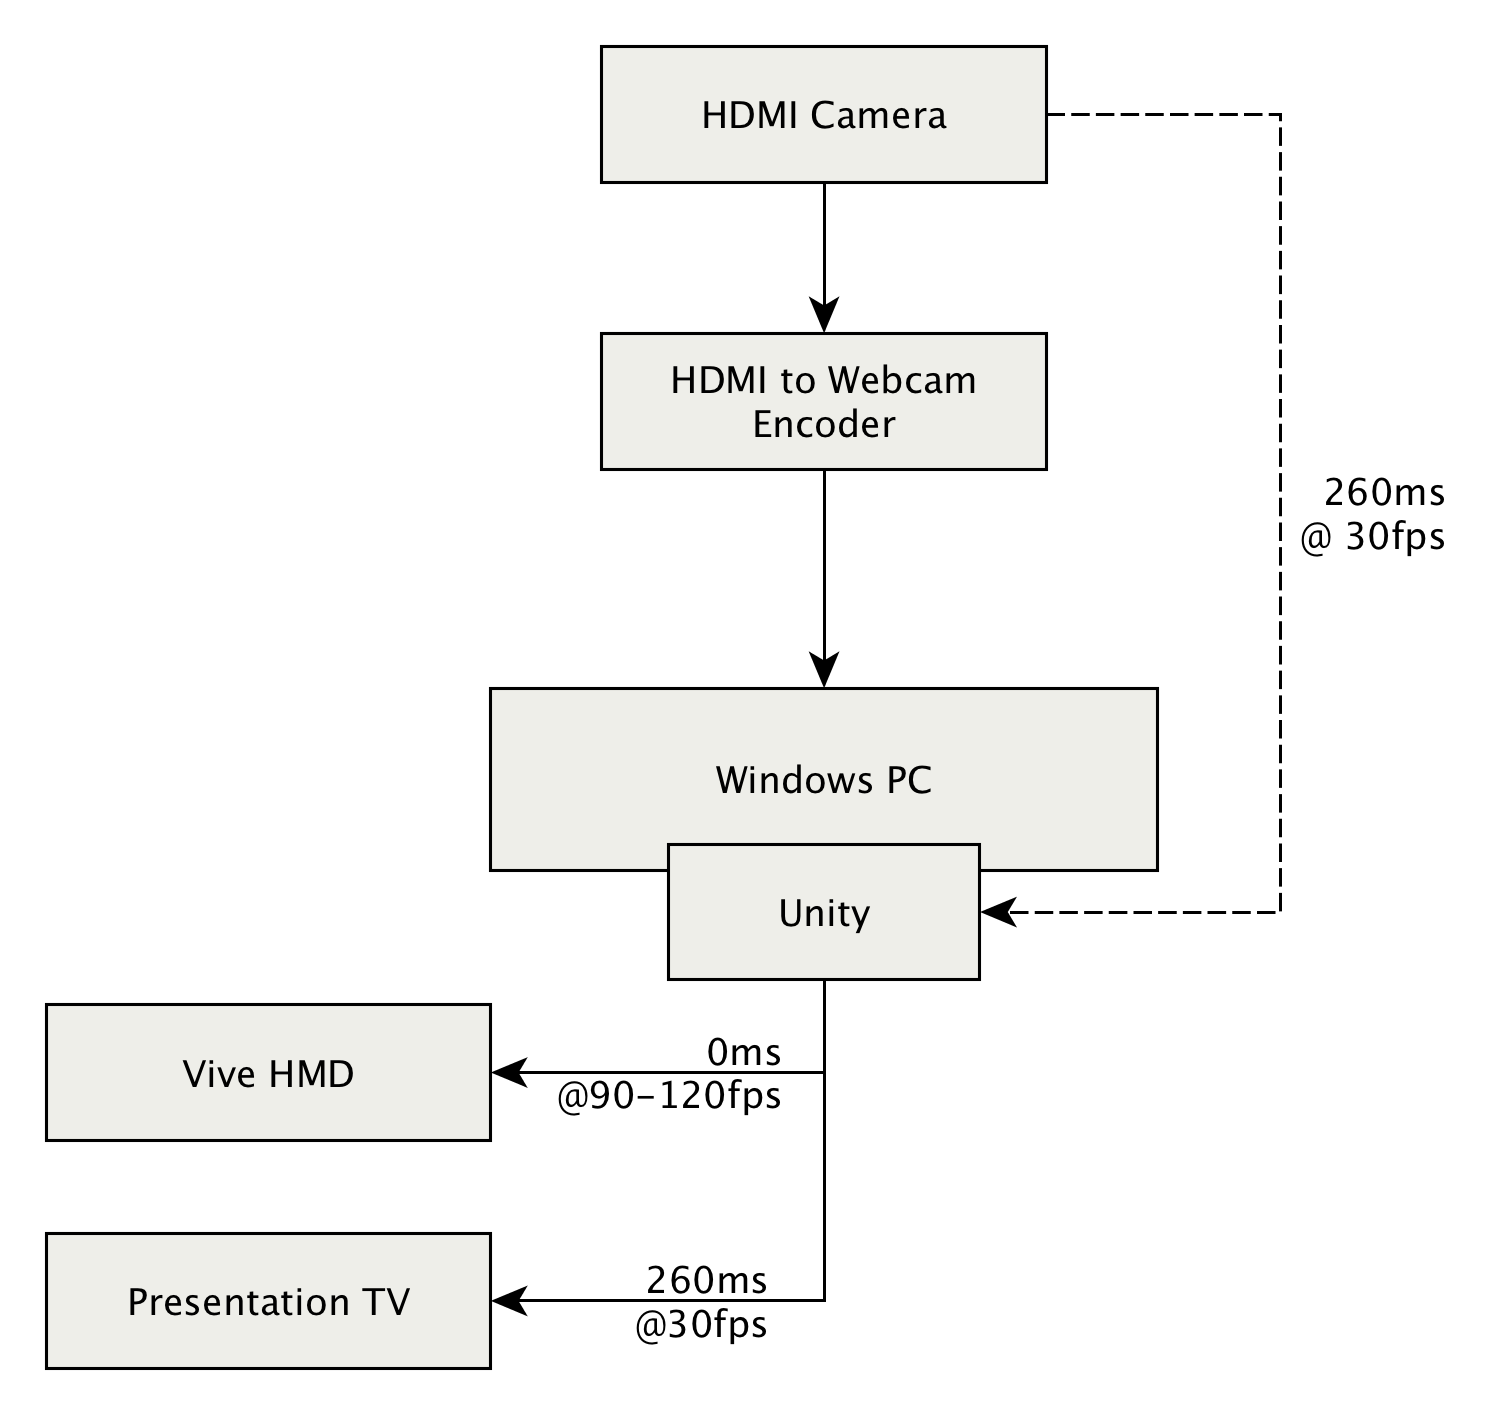
\includegraphics[width=\textwidth]{gfx/FPS-Timing-Components.png}
	\caption{Components in considering timing offsets}
	\label{fig:offsets:components}
\end{figure}

Based on the component diagram \ref{fig:offsets:components} there are two 
important notes: The time offset between camera to Unity and the TV and Vive 
HMD framerate differs. At time of writing Unity does not support dynamic 
framerates on multiple cameras. It is possible to manually initiate a render, 
however, this causes the render loop to mistime and yields to inconsistent 
frame timings inside the HMD.

\todo[inline]{kinda weak text, it's a lot of random words imo}

To conclude: The software has to store a set amount of \gls{framebuffer}s and 
cycle them at the right frame to guarantee minimal delays between camera and 3D 
environment.
\newline

Noteworthy is that the render loop can be 45 or 90 fps, depending on scene 
complexity, slow system performance or - in case of Unity - garbage collection, 
that could halt the engine. To account for this a strategy is needed in which 
Unity's \code{Time.deltaTime} property is used, which describes the time 
between the last and current frame.

\subsection{Framebuffer Swapper implementation}

Unity has a well engineered engine loop. It has a

As initial data needed is \code{cameraFPS}, \code{cameraOffset} and 
\code{Time.deltaTime}. From there it is possible to calculate the remaining 
data for this algorithm:

\begin{lstlisting}
	frameWindow = 1.0 / cameraFPS;
	delayCnt = cameraOffset / frameWindow;
	frameDelay = (int) delay * frameWindow;
	fractionDelay = delay % (1 * frameWindow);
	innerTimer = 0.0;
	absoluteTimer = 0.0;
	while(true) {
		innerTime += Time.deltaTime;
		absoluteTimer += Time.deltaTime;
		localTime = innerTimer - fractionDelay;
		if(localTime < frameWindow ||
		   absoluteTimer < initialDelay) {
			continue;
		}
		
		innerTimer %= frameWindow;
		absoluteTimer %= (1f + initialDelay);
	}
\end{lstlisting}

\todo[inline]{this code listing is the wrong one :( - also I am missing 
representative material why we need to mitigate the latency mitigation}

\subsection{Double Access Ringbuffer}

To spare memory overhead it is possible to reuse previously allocated 
framebuffers. For the final composited image it is necessary that the oldest 
framebuffer is displayed while a new buffer is written into (see Figure 
\ref{fig:offsets:ringbuffer}).

\begin{figure}[htb]
	\centering
	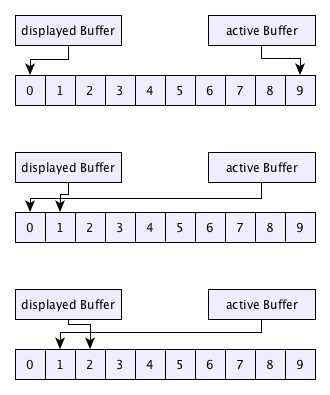
\includegraphics[width=.5\textwidth]{gfx/ringbuffer_schematics.png}
	\caption{Schema of an the ringbuffer}
	\label{fig:offsets:ringbuffer}
\end{figure}

To accommodate for that behavior we have to simply write into the current index 
and display the frame of the next index. After that we increment by one. This 
way we’re overwriting the oldest seen framebuffer and show the one written 
after it.

\begin{lstlisting}
class DoubleAccessRingBuffer<T> {
	public int bufferSize;
	private List<T> buffers;
	private int index;
	
	public DelayedRingBuffer(int bufferSize) {
		this.bufferSize = bufferSize;
		index = 0;
		buffers = new List<long>();
		RebuildBuffers();
	}
	
	public T[] Next(T writeTo, T display) {
		index %= buffers.Count;
		T writeTo = buffers[index];
		T display = buffers[
			(index + 1) % buffers.Count
		];
		if(bufferSize != buffers.Count) {
			RebuildBuffers();
		}
		index++;
		return new T[]{writeTo, display};
	}
	
	void RebuildBuffers() {
		buffers.RemoveAll(_ => true);
		for(int i = 0; i < bufferSize; i++) {
			buffers.Add(new T());
		}
	}
}
\end{lstlisting}

\todo[inline]{Needs "real" pseudo code, rather than implementation}


\section{Mitigating Frame Jitter}

An additional step, that can be handled by the same algorithm, is the 
mitigation of frame jittering. Since the native framerate of the HMD is higher 
than the frames produced by the video feed, there will be noticeable small 
jitters of virtual camera movement, which are not present on the source video 
material. The HTC Vive Controller are very good at picking up minuscule 
changes in motion, which are instantly translated to the transform of the 
camera rig.
\newline
To minimize the effect, it is possible to overwrite framebuffers for as long as 
one duration of a video frame and then swap out these buffers. The headset 
recommends to run it at 90fps - mistimings are no issue either, since it 
results in non noticeable errors in virtual projections while the display frame 
stability and visual performance is unaffected. Thus it is possible to write 
less than three times into a framebuffer, which is mitigated again by 
displaying the final result later - the final image is therefore unaffected.

\todo[inline]{
	That is a bunch of words while not getting to the point.
	\newline
	also needs then lstlisting when the code further up is modified
}
